\documentclass{standalone}
\usepackage{tikz}
\usepackage{ctex,siunitx,bm}
\setCJKmainfont{Noto Serif CJK SC}
\usepackage{tkz-euclide,ninecolors}
\usepackage{amsmath}
\usetikzlibrary{patterns, calc}
\usetikzlibrary {decorations.pathmorphing, decorations.pathreplacing, decorations.shapes,}
\begin{document}
\small
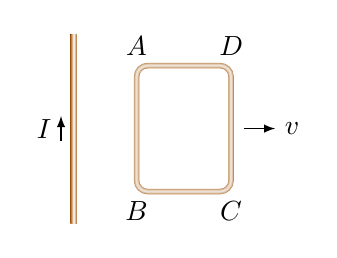
\begin{tikzpicture}[>=latex,scale=0.8]
  \fill[left color=brown5,right color=brown5,middle color=white](-0.05,-1.5)rectangle(0.05,1.5);
  \draw[->](-0.2,-0.2)--(-0.2,0.2)node[midway,left]{$I$};
  \foreach \x in {80,60,40,20}
    {
      \draw[line width={2*sin(\x)},brown5!\x,rounded corners](1.0,1.0)rectangle(2.5,-1.0);
    }
  \node at (1.0,1.0) [above] {$A$};
  \node at (2.5,1.0) [above] {$D$};
  \node at (1.0,-1.0) [below] {$B$};
  \node at (2.5,-1.0) [below] {$C$};
  \draw[->](2.7,0)--(3.2,0)node[right]{$v$};
\end{tikzpicture}
\end{document}